\chapter{Tool Refactoring Methodology}%
\label{methodology}

\section{Architectural Analysis of Packages within RMT}

To understand the operational dynamics of RMT, it is imperative to analyze the codebase, specifically the various packages. The initial phase of the updating process involves discerning the functionality of different code segments to determine whether to undertake a code refactoring or a comprehensive service rewrite.

\subsection{Intermediary Sevice Packages Analisys}
The intermediary service is systematically divided into four main package packages, each comprising functionalities. The first functionality involves the management of refactoring projects. The second pertains to the facilitation of inter-service communication. The third serves as a service discovery mechanism by registering the addresses of all ancillary services to enable seamless subsequent communications. They are illustrated by the package diagram shown in \Cref{fig-package-intermediary}.

\begin{figure}[ht!]
\SetCaptionWidth{\textwidth}
\caption{Intermediary Service Package Diagram}
\label{fig-package-intermediary}
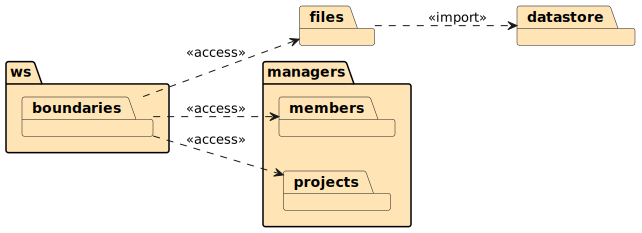
\includegraphics[width =\textwidth, scale=0.2]{Chapter-4/Figures/intermediary-service.png}
\SourceOrNote{Own authorship (2024)}
\end{figure}
\FloatBarrier

The package \verb|datastore| encompasses all configuration files pertinent to the database pool and the connection configuration.

The package \verb|files| contains repository files for database interactions, facilitating queries, insertions, and additional data manipulations.

Within the manager package, the entire outbound logic refers to the refactoring process and the discovery of services, encompassing all related requests for refactoring and generating metrics in the package \verb|managers.projects| and registering the services in the package \verb|managers.members|.

For handling communication, the \verb|ws.boundareis| package includes the controller configurations. Within this package, the bunnies logic is assigned to the persistence and querying of projects and the dispatching of requests to other services. Consequently, this package must access the \verb|managers| and \verb|files| packages.

\subsection{Detection Service Package Analisys}
 
\section{Inicio - Criação de testes}

Me basear no fowler que presa por ter teste unitário antes de modificar para que se possa permanecer o comportamento.

\subsection{Metrics Calculation Service}

\subsection{Detection And Refactoring}

\section{Refatoracao}

\subsection{Refactoring And Metrics Manager Service}

\subsection{Detection And Refactoring Service}

\subsection{Metrics Calculation Service}

\section{Teste da ferramenta}